% 2007 年天津卷理科第 15 题：△ABC 及边 BC 上的点 D（DC = 2BD），连 AD。
% 来源 PDF：source.pdf，SHA256 292db7ce8ca498293125ba6cdb90e0b2c4e41626fe2027f675c7c52b364944df
% 原页：source.pdf 第 1 页（A3 三栏）第 2 栏，书页码 413，图在第 15 题题干下方。
% 重绘依据：题干 ∠BAC = 120° 且 AB:AC = 2:1（原文 "AB = 2AC = 1"，两种读法比均为 2:1，
%   形状不变），取 AB = 2、AC = 1 定形；B、C 置于水平线上，A 在 BC 上方偏 C 一侧
%   （x_A = 5/√7 ≈ 1.890，y_A = √(3/7) ≈ 0.655），D 取 BC 的三等分点（距 B 为 BC 的 1/3），
%   与原图量得的高底比 0.25、BD/BC = 0.33 均吻合。
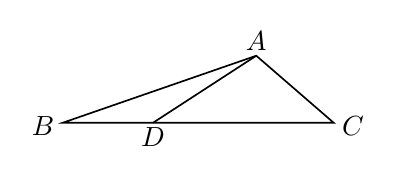
\begin{tikzpicture}[scale=1.3, semithick,
  every node/.style={inner sep=1.5pt}]
  \coordinate (B) at (0,0);
  \coordinate (C) at (2.6458,0);
  \coordinate (A) at (1.8898,0.6547);
  \coordinate (D) at (0.8819,0);
  \draw (B) -- (C) -- (A) -- cycle;
  \draw (A) -- (D);
  \node[anchor=south] at (A) {$A$};
  \node[anchor=east] at ([xshift=-1pt,yshift=-1pt]B) {$B$};
  \node[anchor=west] at ([xshift=1pt,yshift=-1pt]C) {$C$};
  \node[anchor=north] at (D) {$D$};
\end{tikzpicture}
